\documentclass[a4paper, 12pt]{article}
\usepackage[top=2.5cm, bottom=2.5cm, left=2.5cm, right=2.5cm]{geometry}
\usepackage[utf8]{inputenc}
\usepackage{amsmath, amsfonts, amssymb}
\usepackage[portuguese]{babel}
\usepackage{blkarray, bigstrut}
\usepackage{setspace}
\usepackage{graphicx}
\usepackage{amsmath}
\usepackage{tikz}
\usepackage{easybmat}
\newcommand*\circled[1]{\tikz[baseline=(char.base)]{
            \node[shape=circle,draw,inner sep=2pt] (char) {#1};}}


\begin{document}
\begin{center}
Curso de Tecnologia em Sistemas de Computação \\
Disciplina : Probabilidade e Estatística \\
AP2 - Primeiro Semestre de 2020 \\
Nome: Fábio de Oliveira Branco\\ 
\end{center}


\begin{enumerate}
% Questão 1
\item \begin{enumerate}
% Letra a)
\item Para obter a distribuição de probabilidade normalizando a função, precisamos primeiramente integrar a função:\\
$\int_{1}^{3} f(x)dx = \int _1^3\dfrac{1}{4}\left(x-1\right)\left(3x-2\right)dx= \dfrac{1}{4}\times \int _1^3\left(x-1\right)\left(3x-2\right)dx=$\\
$\dfrac{1}{4}\left(\int _1^33x^2dx-\int _1^35xdx+\int _1^32dx\right)= \dfrac{1}{4} \times 3\left[\dfrac{x^3}{3}\right]^3_1 - 5\left[\dfrac{x^2}{2}\right]^3_1 + \left[2x\right]^3_1 =$\\
$\dfrac{1}{4}\left(26-20+4\right) = \dfrac{5}{2}$ \\ 

normalizando a função obtemos o resultado: \\
$f(x)= \dfrac{2}{5} \times \dfrac{1}{4}(x-1)(3x-2) = \dfrac{1}{10}(x-1)(3x-2)$

% Letra b)
\item A fórmula para calcular o valor médio da distribuição é:\\ $$\mu =  \int _{-\infty}^{\infty}x \,\, f(x) \,\, dx$$\\ 
Calculando o valor médio da distribuição através da fórmula obtemos: \\
$\mu = \int _1^3\dfrac{1}{10}x\left(x-1\right)\left(3x-2\right)dx = \dfrac{1}{10}\times \int _1^3x\left(x-1\right)\left(3x-2\right)dx =$\\
$\dfrac{1}{10}\times \int _1^33x^3-5x^2+2xdx =\dfrac{1}{10} \times 3\left[\dfrac{x^3}{3}\right]^3_1 -5\left[\dfrac{x^3}{3}\right]^3_1 + 2\left[\dfrac{x^2}{2}\right]^3_1 =  $ \\
$\dfrac{1}{10}\left(60-\dfrac{130}{3}+8\right) = \dfrac{37}{15} \cong 2,47$

% Letra c)
\item Para calcular a variãncia da distribuição iremos usar a seguinte fórmula: \\
$$\sigma^2 = \int_{-\infty}^{\infty} x^2 \,\, f(x) \,\, dx \,\, - \mu^2$$\\

Calculando o resultado: \\
$\int _1^3\dfrac{1}{10}x^2\left(x-1\right)\left(3x-2\right)dx = \dfrac{1}{10}\times \int _1^3x^2\left(x-1\right)\left(3x-2\right)dx$\\
$\dfrac{1}{10}\times \int _1^33x^4-5x^3+2x^2dx = \dfrac{1}{10}(3\left[\dfrac{x^5}{5}\right]^3_1 - 5\left[\dfrac{x^4}{4}\right]^3_1 + 2\left[\frac{x^3}{3}\right]^3_1) = $ \\
$\dfrac{1}{10}(\dfrac{726}{5} - 100 + \dfrac{52}{3}) = \dfrac{469}{75}$\\ \\
Agora podemos calcular a variância: \\ 
$\sigma^2 = \dfrac{469}{75} -2,47^2 \cong 0,15$ 
\end{enumerate}
%Fim questão 1 
\newpage
% Questão 2
\item \begin{enumerate}
% letra a
\item Para verificar se as expressões são distriuições de probabilidade temos que integrar a função, caso o resultado seja 1  então podemos comprovar que a expressão é uma distribuição de probabilidade. \\

$\int _{-1}^06\left(x^2-1\right)\left(x-x^3\right)dx = 6 \times \int _{-1}^0\left(x^2-1\right)\left(x-x^3\right)dx =$\\
$6\times \int _{-1}^0-x^5+2x^3-xdx = 6\left(-\int _{-1}^0x^5dx+\int _{-1}^02x^3dx-\int _{-1}^0xdx\right) = $\\
$6\left(-\left(-\frac{1}{6}\right)-\frac{1}{2}-\left(-\frac{1}{2}\right)\right) =  1$\\ \\
Verificamos que esta expressão é uma distribuição de probabilidade.\\ 
%letra b
\item $\int _2^4\left(x-3\right)\left(x-2\right)+1dx = \int _2^4x^2-5x+7dx = \int _2^4x^2dx-\int _2^45xdx+\int _2^47dx = $ \\
$\dfrac{56}{3}-30+14 = \dfrac{8}{3}$ \\ \\

Normalizando a função para obter a distribuição de probabilidade: \\
$f(x) = \dfrac{3}{8}(x-3)(x-2)+1$ \\

% letra c
\item $\int _0^1e^x-edx = \int _0^1e^xdx-\int _0^1edx = e-1-e = -1$ \\ \\
Através da integração da função acima percebemos que a expressão não é uma função de probabilidade, pois seu resultado é menor que zero.

\end{enumerate}	
% Questão 3
\item \begin{enumerate}
% letra a)
\item $P(< 39) = P(Z < - 0,095) = 0,5 - 0,0359 = 0,4651$ \\
Resultado aproximado $46,41 \%$ \\
\begin{figure}[!htb]
\centering
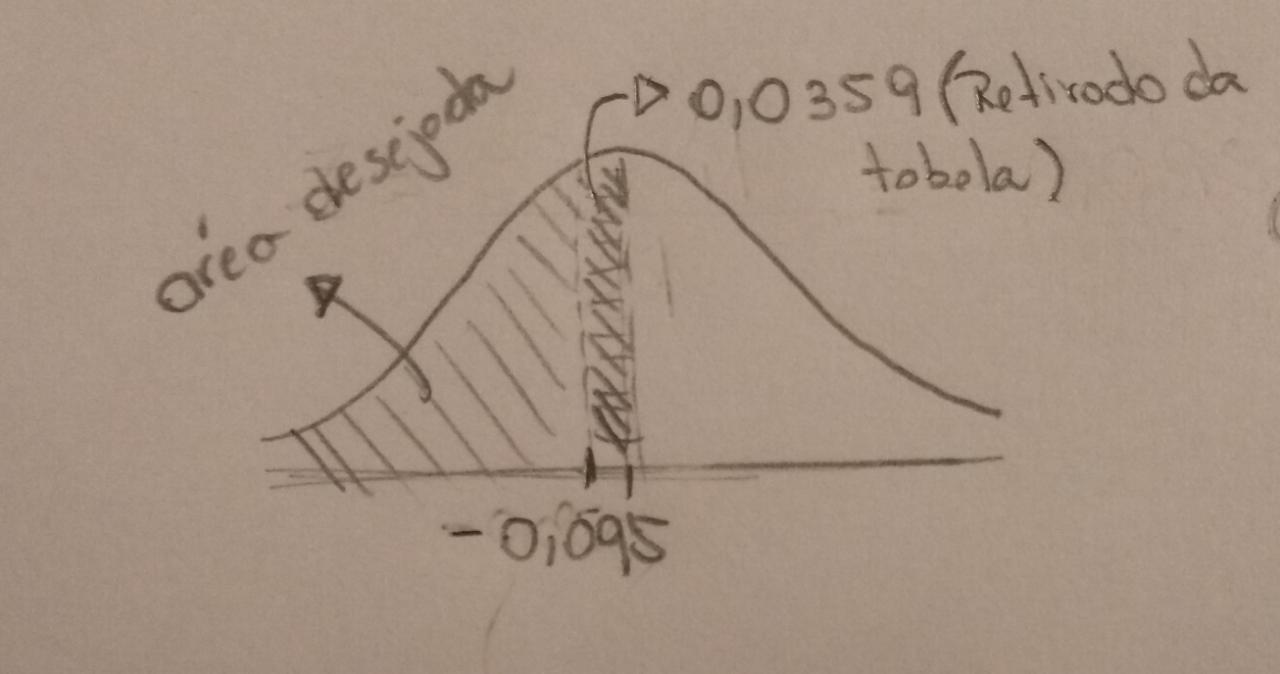
\includegraphics[width=0.5\textwidth]{fotos/figura-1.jpeg}
\end{figure}

\item $P(x > 42) = P(Z > \dfrac{42-41}{21}) = P(Z > 0,0476) = 0,5 - 0,0119 = 0,4801$
Resultado aproximado $48,01 \%$ \\
\begin{figure}[!htb]
\centering
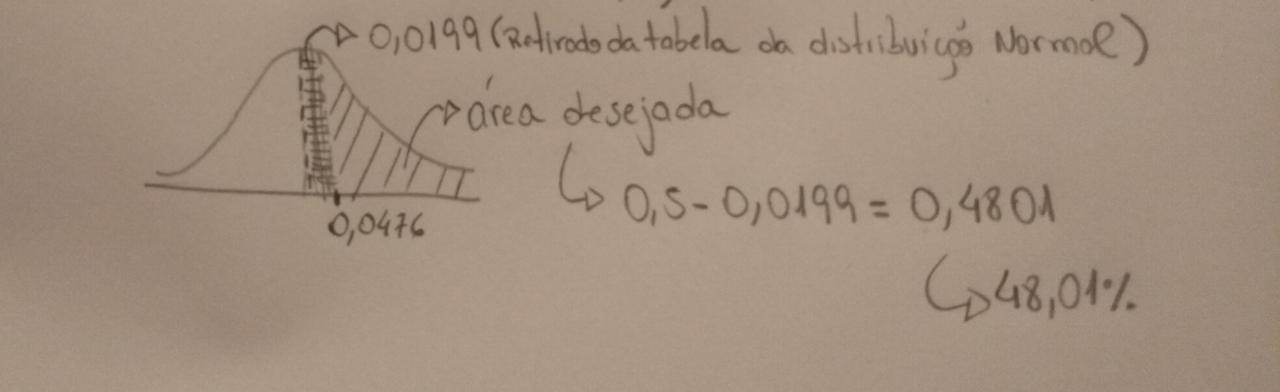
\includegraphics[width=0.5\textwidth]{fotos/figura-2.jpeg}
\end{figure}

\item $C, P(40 < x < 43) = P(\dfrac{40 - 41}{21} < Z < \dfrac{43 - 41}{21}$ \\
$P(-0,0476 < Z < 0,095) = 0,0199 + 0,0359 = 0,0558$ \\
Resultado aproximado $5,58 \%$ \\
\begin{figure}[!htb]
\centering
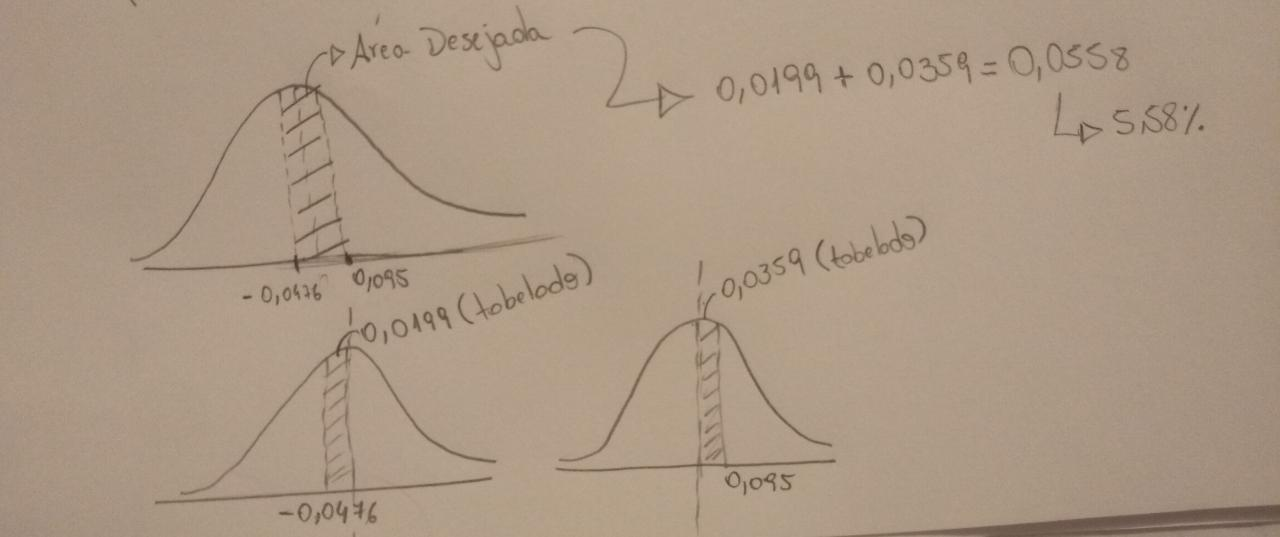
\includegraphics[width=1\textwidth]{fotos/figura-3.jpeg}
\end{figure}

\end{enumerate}

% Questão 4
\item \begin{enumerate}
\item Calculando a média\\ $\mu = \frac{32,8 + 31,1 + 31,9 + 38,9 + 36,0 + 37, 8 + 31,4 + 34,9 + 39, 9 + 33, 2 + 36,8 + 51,4}{12} =  \dfrac{436.1}{12} \cong  36,341$ \\ \\ 

$ l = 32,8^2 + 31,1^2 + 31,9^2 + 38,9^2 + 36,0^2 + 37,8^2 + 31,4^2 + 34,9^2 + 39,9^2 + 33,2^2 + 36,8^2 + 51,4^2 = 16193.1 $ \\ \\
Calculando a estimativa para a variância: \\  $\sigma^2 = \dfrac{1}{11} \times (16193.1 - 12 \times 36,341^2) = \dfrac{1}{11} \times 345.080628 \cong 31,3710$\\
Calculando a raiz quadrada para achar a variância: $\sigma^2 = \sqrt{31,3710} = 5,601$ \\
Aplicando a fórmula para obter o resultado
$IC(\mu, \gamma) = 36,341 - Z_{\frac{95}{2}}\dfrac{5,601}{\sqrt{12}}; X +Z_{\frac{95}{2}}\dfrac{5,601}{\sqrt{12}} = 36,341 - 1,96\dfrac{5,601}{\sqrt{12}}; 36,341 + 1,96 \dfrac{5,601}{\sqrt{12}} $
Resultado $\cong [33,17; 39,51]$

\item Para encontrar a amplitude basta subtrair o valor máximo do intervalo pelo valor mínimo = $39,51 - 33,17 \cong 6.34 $
\end{enumerate}
\item .

\item \begin{enumerate}
\item $\dfrac{1}{10}\times \int _1^{1,4}3x^2-5x+2dx = \dfrac{1}{10} \times \int _1^{1,4}3x^2dx-\int _1^{1.4}5xdx+\int _1^{1,4}2dx \cong 0,014$
\item $media = 21,6, \,\,\, variancia = 7,42$\\
$P(\dfrac{23,4-21,6}{\sqrt{7,42}} <Z< (\dfrac{26,7-21,6}{\sqrt{7,42}}) \cong 0,660 < Z < 1,87$\\
$P(1,85< Z) - P(0,66 < Z) = 0,4693 - 0,2454 \cong 0,223$
\item $P(X > 1,9) = e^{-1,721 \times 1,9} = 0,038 $
\item $P(X < 1,9) = \dfrac{1}{6,3 - 1,2} \times \int _1^{1,9} \cong 0,176
$
\end{enumerate}
\end{enumerate}

 
\end{document}
